\documentclass{icmmcm}

\usepackage{url}
\usepackage{graphicx}
%\usepackage{listings}

\newcommand{\der}{\mathrm{d}}

\title{The Mathematical Model of the Optimized Use of Ebola Virus Drug}
\team{38403}
\question{A}
%\date{February 8, 2015}

\begin{document}
\begin{summary}
A new medication may prevent the spread of Ebola virus and cure
 those patients in the early affected period. How to make full
 use of the new medication to fight Ebola is of great concern
 and top priority. We are going to establish two mathematical
 models: one to predict  the infection trend of Ebola virus, the
 right quarantine time and appropriate dosage; the other to
 explore the optimal distribution  in transportation systems and
production rate.
\par Model One will center on Ebola virus infection trends,
 quarantine time and the amount of medication. According to the
 characteristics of Ebola virus transmission, An Ordinary 
 Differential Equation (ODE) model of virus transmission is
 built, along with the relevant graphics. On the basis of phase
 trajectories, discussions are made about the nature of ODE
 model of the spread of disease, the entire process of virus
 transmission and the best time for initial virus isolation is
 calculated. A nonlinear regression analysis is performed to
 test the reliability of the model.
\par Model two will explore the optimal medication distribution
 within transport systems and the optimal drug production rate.
 Some specific mathematical models are created by linear
 programming in order to save the transportation time.
\end{summary}

\maketitle
\thispagestyle{fancy}

%%% Uncomment the following lines if you have figures or tables in
%%% your report:
%% \listoffigures
%% \listoftables

\section{Introduction}
\subsection{The basic situation of Ebola virus}
 Ebola is a cause in humans and other primate and mammals, with
 a high mortality rate of 50\% to 90\% \cite{bib1}. It is of
 great importance to develop an effective medicine. World
 Medication Association declared that the newly develop drugs
 can cure the less seriously affected patients. Therefore the
 key of our model is to help with the effective use of the
 life-saving drugs.
\subsection{The Direction of Research}
The main direction of our research is to use a variety of
mathematical methods and means to achieve the optimal use 
of the drug and the full value of drug, thereby reducing the
Ebola virus infection rate and mortality.
\section{Problem Analysis}
\subsection{The Restatement of the Problem}
Ebola virus appeared resulted in the death of many patients,
the Medical Association developed a drug to cure patients yet
to come late, so that more patients get second chance to see
the hope of life.
\par The model we build contributes to the crucial role the 
medicines play at the moment.
\par Factors that play a crucial role in the influence of drugs,
including the speed of the disease, isolation time, the amount
of drug required drug, delivery systems and drug production
speed. Thus our tasks are gradually clear.
\par The task is as follows:
\begin{itemize}
  \item The establishment of the Model One is to be more
  intuitive to see the trends in the spread of Ebola virus.The
  model not only provides important information for Ebola
  virus' prevention and treatment but also a similar model for
  the spread of other virus.
  \item Using the conclusion of Model One, we can calculate the
  isolation time roughly and then calculated the drug dosage
  further.
  \item Searching the database of the infected cases and using
  the nonlinear regression ``nlinfit'' analysis to test the
  reliability of Model One.
  \item The establishment of the Model Two is to explore the
  best transportation system for drug distribution, so that we
  can save drug delivery time and strive to save more patients.
  \item Using the Model Two elaborating the drug delivery rate
  and drug production speed is to calculate vaccines and drugs
  production speed.
  \item Using the speed of medicine transport and 
  production in Model Two to further calculate the rate of
  vaccine and medicine production.
\end{itemize}
\subsection{The Layout of Problem Solving}
\begin{itemize}
  \item First of all, we need to establish the ordinary
  differential equation models of the spread of Ebola
  virus(Model One), draw images, describe
  propagation of Ebola virus and discuss the characteristics
  concerned the solution. At the same time, using of the model
  we can calculate the best time to isolate rough.
  \item Secondly, use the results of Model One to identify
  positive relationship between dosage and the number of
  infections including time parameter variables, and then we
  can calculate the total dose.
  \item Thirdly, according to the database provided by World
  Health Organization(WHO), drawing scatter plots and using the
  nonlinear regression ``nlinfit'' analysis to test the
  reliability \cite{bib6}.
  \item Fourthly, using linear programming model in the use of
  transport,we establish transport system of Ebola drug.
  \item Fifthly, using the results of optimal transport from
  Model Two to determine the nonlinear relationship between
  production rate and optimal distribution and calculate the
  vaccine and medicine production rate.
  \item Finally, according to the results of our research,
  write a non-professional letter for the World Medical
  Association's announcement.
\end{itemize}

\section{Model Design}
\subsection{The Spread of the Ebola Virus}
\label{sec:m1}
For convenience, we defined some symbols:
\begin{center}
\begin{tabular}{|r|p{7cm}|}
\hline
$ i(t) $ & total cases on $t$-th day.\\
\hline
$ i(0)=i_0 $ & total cases on beginning.\\
\hline
$ N $ & population in this area.\\
\hline
$ k $ & infect factor\\
\hline
$ r(t) $ & number of people exited from the epidemic process on
$t$-th day.\\
\hline
%$ p_0 $ & \\
%\hline
\end{tabular}
\end{center}%
\textbf{\large Modeling:}\\
\textbf{Case 1:}\\
Assumptions:
\begin{enumerate}
  \item There is no body recover or die in the present period.
  \item Population $ N $ remain unchanged, it means
  that we don't care population death,birth and flow.
  \item Take $ k_0 $ as the number of people infected by
a patient in one day.
%  \item The ebola virus no variation in the present period.
\end{enumerate}
The increasement of cases from $ t $ to $ t+\Delta t$ is:
\begin{equation}
i(t+\Delta{t})-i(t)=k_0i(t)\Delta{t}
\label{equ:1}
\end{equation}
we can get a ordinary differential equations model for 
equation (\ref{equ:1}):
\begin{equation}
\left\{
\begin{array}{l}
\frac{{\der}i(t)}{{\der}t}=k_0i(t)\\
i(0)=i_0
\end{array}\right.
\label{equ:2}
\end{equation}
the solution of equation (\ref{equ:2}) is:
\begin{equation}
i(t)=i_0e^{k_0t}
\label{equ:3}
\end{equation}
the figure of equation (\ref{equ:3}) is Figure~\ref{fig:1}:\par
\begin{figure}
\centering
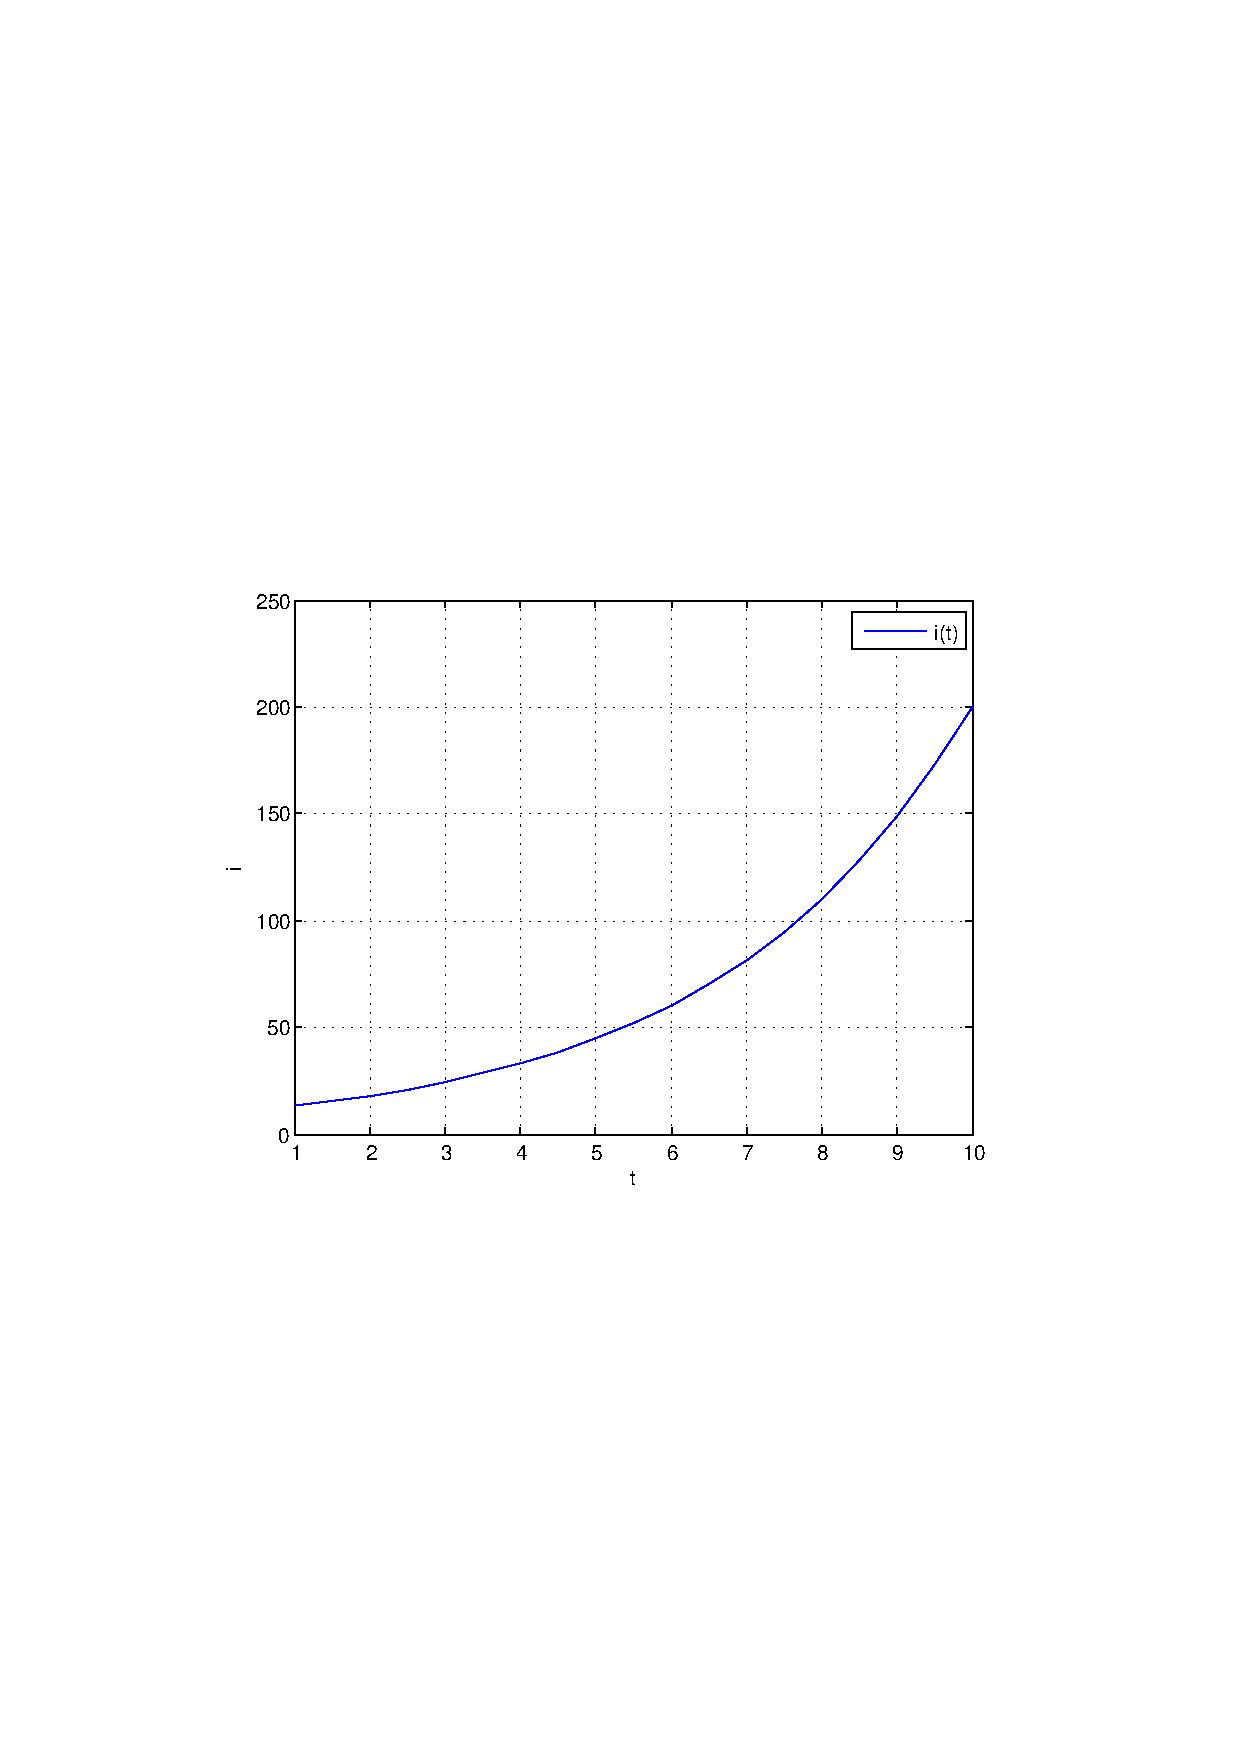
\includegraphics[width=4in]{imgs/i(t).pdf}
\caption{Spread of Ebola virus.}
\label{fig:1}
\end{figure}
Figure~\ref{fig:1} shows us that: 
The Ebola virus spread increases exponentially.
The results are in good agreement with 
the Ebola virus spread in beginning, in general, Ebola
spread speedy in beginning, the infected person growth in the
exponential function, when $t$ tends to infinity, then $i(t)$
tends to infinity. But the actual situation of the Ebola virus
late is not fit, because in the patients's effective
contact crowd, have healthy people and patients, while only
health personnel can be infected. And part of patients will die
in this period.\par
Improve this model, then we have case 2.\\
\textbf{Case 2:}\\
Assumptions:
\begin{enumerate}
  \item Assuming infected and cured with long-term immunity,
   does not consider the case of long-term repeated infections,
   healthy immediately after infection can become infected
   persons. In this case, the people of the entire region is
   divided into three categories: The first category is
   contagium which able to infect others, indicating
   the number of such moment $ t $ with $ i(t) $; second
   category is susceptible which vulnerable to becoming infected, 
   with $ s(t) $ represents the number of such moment $ t $;
   the third category is a person other than the two
   categories above, including death after infection,
   get a long-term immunity after illness, who are
   no longer infected, represents the number of such
   moments $ t $ with $ r(t) $.
  \item The region's total population $N$ remain unchanged
   during the discussion, that is not considered births, deaths,
   flow and so on.
  \item The speed of change from first class to second class is
   proportional to the number of first class.
\end{enumerate}
\begin{equation}
k=\frac{k_0}{s(t)}
\label{equ:4}
\end{equation}

\begin{equation}
l=\frac{\frac{{\der}r(t)}{{\der}t}}{i(t)}
\label{equ:5}
\end{equation}

\begin{equation}
\left\{
\begin{array}{l}
\frac{{\der}r(t)}{{\der}t}=li(t)\\
\frac{{\der}i(t)}{{\der}t}=ks(t)i(t)-\frac{{\der}r(t)}{{\der}t}\\
\frac{{\der}s}{{\der}t}=-\frac{{\der}i(t)}{{\der}t}-\frac{{\der}r(t)}{{\der}t}
\end{array}\right.
\label{equ:6}
\end{equation}%
%
where $ i(0)=i_0,s(0)=s_0,r(0)=r_0=N-i_0-s_0 $.
%
\begin{equation}
\left\{
\begin{array}{l}
\frac{{\der}i(t)}{{\der}t}=ks(t)i(t)-li(t)\\
\frac{{\der}s(t)}{{\der}t}=-ks(t)i(t)\\
\frac{{\der}r(t)}{{\der}t}=li(t)\\
i(0)=i_0,s(0)=s_0,r(0)=r_0=N-i_0-s_0
\end{array}\right.
\label{equ:7}
\end{equation}
\begin{figure}
\centering
\includegraphics[width=4in]{imgs/sars3_2.pdf}
\caption{Phase trajectoriesthe for equation (\ref{equ:7})}
\label{fig:2}
\end{figure}
Equation (\ref{equ:7}) is difficult to obtain an accurate
solution, can be the first to make numerical calculations.\par
  Numerical calculation: For convenience of calculation, visual
$ s(t) $ and $ i(t) $ is the proportion of the total number,
and therefore, in equation (\ref{equ:7}), set $k=1$,
$l=0.5$, $i(0)=0.01$, $s(0)=0.80$, using MATLAB software
programming as appendix 1 and 2, product Figure~\ref{fig:2} for
$i(s)$.On the phase plane s-i, the domain of the phase
trajectories is $ D=\{(s,i),s>0,i\geq 0,s+i\leq1\} $.\\
Elimination $ t $, then:
\begin{equation}
\frac{{\der}i}{{\der}s}=-1+\frac{1}{ks}
\label{equ:8}
\end{equation}
Set $\rho=1/k$, said $\rho$ is a characteristic (on the
same area and the same infectious,$\rho$ is a constant).
\begin{equation}
\frac{{\der}i}{{\der}s}=\frac{\rho}{s}-1
\label{equ:9}
\end{equation}

\begin{equation}
i(s)=\rho lN\frac{s}{s_0}-s+s_0+i_0
\label{equ:10}
\end{equation}

Draw its figure:\par
\begin{center}
\includegraphics[width=4in]{imgs/i(s)_i_s.pdf}
\end{center}

From this figure, we can see that:
\begin{enumerate}
  \item regardless of where the phase trajectoriesthe start on,
   it will eventually intersect with the $s$ axis,
   that is the patient will eventually disappear;
  \item the final uninfected healthy proportion is
   $s_m$(when $t\rightarrow\infty$);
  \item if $s_0>\rho$, the $i(t)$ first increase, while when 
   $s=\rho$, $i(t)$ reaches a maximum:
   $$
	i_m=s_0+i_0-\rho(1+lN\frac{s_0}{\rho})
   \label{equ:11}
   $$
   Then, $i(t)$ decreases and tends to zero, $s(t)$ is
   monotonically reduced to $s_m$.
  \item If $s_0<\rho$ then $i(t)$ decreases monotonically to
   0, $s(t)$ decreases monotonically to $s_m$.
\end{enumerate}
The following study relationship between Ebola virus spread and
time of begin taking isolation.\par
\begin{figure}\centering
\includegraphics[width=4in]{imgs/iso_i_t.pdf}
\nline%
(A)
\\\nline%
\includegraphics[width=4in]{imgs/iso_i_s.pdf}
\nline%
(B)
\caption{The effect of different time of begin taking 
isolation for spread.}
\label{fig:4}
\end{figure}
The figure below is based on Figure~\ref{fig:2} with changeing
the time when start taken to isolate, when $l$ will increase.
Figure~\ref{fig:4}(B) is the effect of different time of begin taking 
isolation for the number of patient, $1,2,\cdots,n$ hour
corresponding image by the bottom-up.(MATLAB code for this part
is in appendix 1, 3 and 4)\par
As can be seen from Figure~\ref{fig:4}(A), with the start of
the time taken to isolation increasing, from the dense
continuous curve becomes too sparse, that is, at the time of
virus infection, in a certain period of time, little change in
the number of infected, but in the longer time to take
isolation, the number of infections is growing rapidly.
As can be seen from Figure~\ref{fig:4}(B), when began to take
isolated relatively in short time , the maximum number of
infections is relatively small, but with a long time, the sharp
increase in the number of infections. So once found infected
should be isolated as soon as possible, in 4h hours of isolation
is ideal, relatively small number of infections infected by per
patient, but if it start take isolation than 11h, then the
consequences will not optimistic, each patient infect
a lot of people.



\subsection{Required Drug}
Symbol definition:
\begin{center}
\begin{tabular}{|r|p{8cm}|}
\hline
$ p_0 $ & In the cure range, the maximum dosage required to
cure Ebola patients.\\
\hline
$ Q(t) $ & The amount of drug at time $t$.\\
\hline
\end{tabular}
\end{center}%
Assumptions:
\begin{enumerate}
  \item The ebola virus no variation in the present period.
\end{enumerate}
The amount of the drug required to $ Q(t)=p_0*i(t) $.\par
The figure for $ i(t) $ in Case 2 shown as below:
\begin{center}
\includegraphics[width=4in]{imgs/sars3_1.pdf}
\end{center}
The amount of drug $Q(t)$ can be calculated is $p_0$ times of
$i(t)$, $Q(t)$ change with $t$ similar to $i$ change with $t$.

\subsection{Transportation System}
Assumptions:
\begin{enumerate}
  \item Because the number of patients increase with time in the short
term, to make patients whose illness is not serious can be
cured, the speed of the drugs production $ v(t) $ needs
increasing with time.
  \item Drug delivery using the same kind of transportation and
transportation speed is $ v_0 $.
  \item There are $ m $ production places $ A_1,A_2,\cdots,A_m $
for the drug,the producting speed for the drug of $ A_i $ is
$ a_i $,$ i=1,2,\cdots,m $.There are $ n $ places $
B_1,B_2,\cdots,B_n $ need the drug,the demand of $ B_i $ is
$ b_i $,$ i=1,2,\cdots,n $.
  \item $ \sum_{i=1}^{m}a_i=\sum_{j=1}^{n} $.For all
$ i\in\{1,2,\cdots,m\} $ and $ j\in\{1,2,\cdots,n\} $, have
$ a_i,b_j>0 $.
$ x_{ij} $ is the quantity of drug transported from $ A_i $ to
$ B_j $,and $ s_{ij} $ is the transportation path length from
$ A_i $ to $ B_j $.
\end{enumerate}\par
The problem is how to determine the optimal transportation
scheme:
Ensure supply, make the shortest transportation time.\\
The mathematical model for the problem is:\\
Drug production time $ t=\frac{x_{ij}}{v(t)} $, drug
transportation time $ t'=\frac{s_{ij}}{v_0} $, let
$ c_{ij}=\frac{1}{v(t)} $, then:
\begin{equation}
min t=\sum_{i=1}^{m}\sum_{j=1}^{n}(t+t')=
\sum_{i=1}^{m}\sum_{j=1}^{n}c_{ij}x_{ij} + 
\sum_{i=1}^{m}\sum_{j=1}^{n}t'
\label{equ:31}
\end{equation}
$$
s.t. \left\{
\begin{array}{l}
  \sum_{j=1}^{n}x_{ij}=a_i,i=1,2,\cdots,m \\
  \sum_{i=1}^{m}x_{ij}=b_j,j=1,2,\cdots,n \\
  x_{ij}\geq 0,i=1,2,\cdots,m, j=1,2,\cdots,n
\end{array}\right.
$$
where $ \sum_{i=1}^{m}\sum_{j=1}^{n}t' $ is certain, 
we just calculate the minimum of 
$ \sum_{i=1}^{m}\sum_{j=1}^{n}c_{ij}x_{ij} $.\\
Let:
$$
\begin{array}{ll}
x & = ~\begin{pmatrix}
	  x_{1,1} & x_{1,2} & \cdots & x_{1,n} \\
	  x_{2,1} & x_{2,2} & \cdots & x_{2,n} \\
	  \vdots  & \vdots  & \ddots & \vdots  \\
	  x_{m,1} & x_{m,2} & \cdots & x_{m,n}
	 \end{pmatrix}\\\\
C & = ~\begin{pmatrix}
	  c_{1,1} & c_{1,2} & \cdots & c_{1,n} \\
	  c_{2,1} & c_{2,2} & \cdots & c_{2,n} \\
	  \vdots  & \vdots  & \ddots & \vdots  \\
	  c_{m,1} & c_{m,2} & \cdots & c_{m,n}
	 \end{pmatrix}\\\\
b & = ~\begin{pmatrix}
	  a_1 & a_2 & \cdots & a_m & b_1 & b_2 & \cdots & b_n
	 \end{pmatrix}\\\\
A & = ~\begin{pmatrix}
	  a_{1,1} & a_{1,2} & \cdots & a_{1,n} \\
	  a_{2,1} & a_{2,2} & \cdots & a_{2,n} \\
	  \vdots  & \vdots  & \ddots & \vdots  \\
	  a_{m,1} & a_{m,2} & \cdots & a_{m,n}
	 \end{pmatrix}
\end{array}
$$
where $ a_{ij}=e_i+e_{m+j} $, $ e_{i} $ is a column vector with
$ m+n $ elements, and i-th element is 1, otherwise 0. Then we
have:
$$
min z=Cx
$$
$$
s.t. \left\{\begin{array}{r}
  Ax=b\\
  x\geq 0
\end{array}\right.
$$
when $ \sum_{j=1}^{n}x_{ij}=a_i $, we can ensure the
availability of drugs in different place.
\subsection{Produnction Speed}
Symbol definition:
\begin{center}
\begin{tabular}{|r|p{8cm}|}
\hline
$ x_{ij} $ & The quantity transport from $ A_i $ to
$ B_j $.\\
\hline
$ v(t) $ & The speed of the drug production at moment $t$.\\
\hline
$ t $ & Time in production.\\
\hline
$ t' $ & Time in transportation.\\
\hline
\multicolumn{2}{|c|}{$ i=1,2,\cdots,m;j=1,2,\cdots,n $}\\
\hline
\end{tabular}
\end{center}%
$v(t)=\frac{x_{ij}}{t-t'}$, according to the formula, to obtain
the shortest transportation time $t$($t>t'$), we can find the
maximum production speed.

\section{Testing and Analysis}
\subsection{Model Testing}
Now take cases infected with Ebola in the distribution of West
African countries as an example \cite{bib5}(data see appendix
6), by each set of data, the number of days as the horizontal
and the number of infections to the vertical axis, to make a
scatter plot, as shown in Figure~\ref{fig:5}(A).
\begin{figure}
\centering
\includegraphics[width=4.7in]{imgs/sum_anly.pdf}
\caption{Statistic data and fitting}
\label{fig:5}
\end{figure}
Using MATLAB Statistics Toolbox function nlinfit, fitting
formula according to data:
\begin{equation}
i(t)=113e^{0.01748t}+0.2253e^{0.05946t}
\label{equ:14}
\end{equation}
The formula in line with graphs for Ebola
virus infection early on the case 2 in Section~\ref{sec:m1},
from Figure~\ref{fig:5}(B) we can see the data fit with good
results. It show that these assumptions and models
introduced is appropriate.
\subsection{Model Analysis}
Analyze data on the distribution of infection cases by Ebola 
in the West African countries and make fitting bias figure, as
shown in Figure~\ref{fig:6}.\\
\begin{figure}
\centering
\includegraphics[width=4in]{imgs/cases_fit_bias.pdf}
\caption{Bias analyze.}
\label{fig:6}
\end{figure}
As can be seen from Figure~\ref{fig:6}, the error branch points are
concentrated in the interval $[-55,55]$, so fitting fine,
it shows that the function above in line with the increasement
trend of infectious diseases on beginning, the model has good
fidelity.(MATLAB code for this part is in appendix 5)


\section{Model Evaluation}
\subsection{Advantage}
\begin{itemize}
  \item This model gives a result of a general, not only for
  Ebola virus infection case analysis, but also for other
  infections virus analysis.
  \item Model use a method of combination of numbers and shapes
  to present Ebola virus propagation visually objectively.
  \item Model了not only takes into account more than two origin,
  more requirements to the case  but also combines drug
  production speed with drug delivery speed to get the optimal
  allocation scheme.
  \item The model takes into account the recovered cases and
  death (no more infection) and greatly improve the
  predictability and applicability of the model.
  \item The principle of the model is straightforward. It
  simplify algorithm. Model has good practicability.
\end{itemize}
\subsection{Weaknesses}
\begin{itemize}
  \item The study population N is the total number of dynamic
  change, there is birth, death, flow and so on. This makes the
  model and the actual situation have a tolerance.
  \item Ebola virus in the human body have latency and Ebola
  virus carriers is not contagious, and this is where the model
  is not perfect.
  \item  Drug has half-life in human body. Patients must adhere
  to medication for some time to recover, so the dose
  calculations and the actual have a tolerance.
  \item Several factors are not taken into account, such as
  technology level of every medicine manufacturer, the
  different production rate and difference in transport
  vehicle, road condition, which might result in the gap
  between optimal distribution plan and the reality.
  \item In actual circumstances, defective medicines in
  production, in transport and in medicine-taking will affect
  the reliability of the model.
\end{itemize}
\subsection{Improvement and Value of the Model}
In the process of model predictions, program one in Model One
ignores many factors, does not comply with the later development
of Ebola virus infection. Based on program one, we consider more
factors and then establish program two. Development of Ebola
virus infection and the development of other infections were
similar. However we know that both the use of drug and isolation
measures for Ebola virus infection trend have important
effect. Therefore, our model can give a more comprehensive
account of multiple factors and address the real problems. In
other words, the model prediction in the number of infections is
accurate, but due to virus variation and other uncontrollable
factors, it might not be predicable in the long period. To
develop in line with the actual situation of the Ebola
virus-term forecast, we must improve the above model further.
\par Model two are simplified in many factors, so our model
should consider all factors affecting the transport logistics
and distribution, but the reality is very complex,multifaceted
consideration is needed to improve our model of development
direction.
\par Generally, infection intensity can be perceived through
the new added cases between intervals yet the infection trend
can hardly be determined. The model we build can solve the
problem and present a clearer picture of the transmission and
seize the best time to quarantine. In terms of distribution and
transport, our model can calculate the shortest time of
transport and production, hence saving more time and life by
providing medicine to disease-stricken areas.
Our model can be applied not only to the
establishment of the Ebola virus, but also be applied to a virus
similar to Ebola.

\section{A Letter for the World Medical Association}
\centerline{A letter for the World Medical Association}
Dear the World Medical Association:
\par Thanks to the world medical association has manufactured a
new medication for the treatment of Ebola virus to control the
spread of Ebola, more and more patients can be treated. In
order to make better use of the medication, we also need to
optimize the amount of drugs, drug distribution transportation
systems, drug production speed.
\par According to our research, we got two findings from our
research and modeling. In terms of the trends of Ebola virus
infection, we find that Ebola cases will continue to increase
dramatically if no control is made at early stage, but
infection can be control if prevention is made such as
therapeutic agents. When drug application is optimized,
infection will cease, even decline. Also, the infection will
spread only when the number of infected cases is over a certain
threshold. That's why Ebola transmit more rapidly in those
densely-populated areas, where prevention is poorly managed and
excluding rate is high. Reversely, Ebola can be better
controlled in less populated areas with a lower infection rate.
In terms of drug dosage, we must make sure sufficient medicine
supply for early infected patients but avoid possible wastes.
The dosage of most severe cases is used as the base and
multiplied by the number of patients. The calculated result is
the best dose.
\par We also studied the best drug distribution transport
systems. The purpose is to guarantee the amount of medicine for
each infected areas and fast acquisition of the medicine. Given
that the needed amount and production volume is constant, we
calculate the minimum time for medicine production and the
amount of time for distribution. This is the best distribution
plan that can save more time and lives. Regarding the
production rate, the amount of needed medicine divided the time
spent in production is the best production rate.
Mentioned above is the result of our study. We hope that the
World Medical Association will seriously consider and adopt the results of our study, and
show an announcement on better optimize the use of drugs in
order to do a better job in the fight against Ebola!
\par Our team wishes Ebola patients can recover rapidly and
people all around the world are happy and healthy!\\\nline%
\rightline{Team \#38403}
\rightline{February 9, 2015}

\bibliographystyle{plain}
\begin{thebibliography}{10}
\bibitem{bib1}Ebola virus, Baidu Encyclopedia,
  \url{http://baike.baidu.com/subview/188032/5072671.htm}

\bibitem{bib2}Wei Li, On Mathematical Model of the Spread of
  SARS Virus, Journal of Bijie Teachers College (volume 22,
  issue 2, June 2004)

\bibitem{bib3}Jiang Hua,Pan Haixia,\ldots, Simulating the Ebola
virus disease transmission and outbreak in China by using computational
epidemiological model, Chinese Journal of emergency
medicine(volume 23, issue 9, September 2014)

\bibitem{bib4}Xueqin Wu,Linear Programming in logistics and
transportand application of mathematical models, Journal of
Jiangxi Vocational and Technical College of Electricity(volume
20, issue 1, March 2007)

\bibitem{bib5}The latest data of deaths from Ebola,
\url{http://snap.windin.com/ns/findsnap.php?id=232970537}

\bibitem{bib6}Shaohui Zhang, The mathematical model, Science
Press(August 2010)
\end{thebibliography}

\section*{Appendix}
\textbf{1.MATLAB code for function ill (ill.m):}
\begin{lstlisting}[language=Matlab]
function y = ill(t,x)
k=1;l=0.5;
y=[k*x(1)*x(2)-l*x(1);-k*x(1)*x(2)];
end
\end{lstlisting}\nline%
%
\textbf{2.MATLAB code for solve ill (sill.m):}
\begin{lstlisting}[language=Matlab]
ts=0:50;
x0=[0.01;0.80]
[t,x]=ode45('ill',ts,x0);[t,x]
figure(1);
clf;
hold on;
plot(t,x(:,1),'-r','LineWidth',2);
plot(t,x(:,2),'-.b','LineWidth',2);
plot(t,1-x(:,1)-x(:,2),'--g','LineWidth',2);
xlabel('t');ylabel('i,s,r');
legend('i(t)','s(t)','r(t)');grid on;%pause
figure(2);
plot(x(:,2),x(:,1),'LineWidth',2);
xlabel('s');ylabel('i');
legend('i(s)');
grid on;
hold off;
\end{lstlisting}\nline%
%
\textbf{3.MATLAB code for function ill2 (ill2.m) when taken
isolution:} \begin{lstlisting}[language=Matlab]
function y = ill2(t,x)
k=1;l=0.6;
y=[k*x(1)*x(2)-l*x(1);-k*x(1)*x(2)];
end
\end{lstlisting}\nline%
%
\textbf{4.MATLAB code for study the effect of different time of
begin taking isolation for spread:}
\begin{lstlisting}[language=Matlab]
dur=50;
ts=0:dur;
x0=[0.01;0.90];
figure(1);
[t,x]=ode45('ill',ts,x0);
plot(t,x(:,1),'r-.');
xlabel('t');ylabel('i');
hold on;
figure(2);
clf;
plot(x(:,2),x(:,1),'r*-.');
hold on;
for g=1:(dur/3)
    [t,xx]=ode45('ill2',ts((g+1):dur),x(g,:));
    figure(1);
    plot(t,xx(:,1));
    figure(2);
    plot(xx(:,2),xx(:,1));
end
xlabel('s');ylabel('i');
legend('no isolation','isolation');
hold off;
figure(1);
legend('no isolation','isolation');
hold off;
\end{lstlisting}\nline%
%

\end{document}
